\section{Running an example}
As an example, we will consider the following situation. Two islands have been colonized by a species originating from a continent. We have three samples, one from the continental population (population 1) and one from each of the two islands (population 2 and 3). We consider three possible scenarios :
\begin{description}
\item[scenario 1] : one island (population 2) was first colonized by migrants from the continent (population 1) and the second island (population 3) was subsequently colonized by migrants from the first island (population 2),
\item[scenario 2] : same as scenario 1 but swaping the two island populations,
\item[scenario 3] : the two islands were colonized independently by migrants from the continent.
\end{description}
This can be illustrated by the following figure :
\begin{figure}[h]
\begin{center}
\begin{tabular}{ccc}
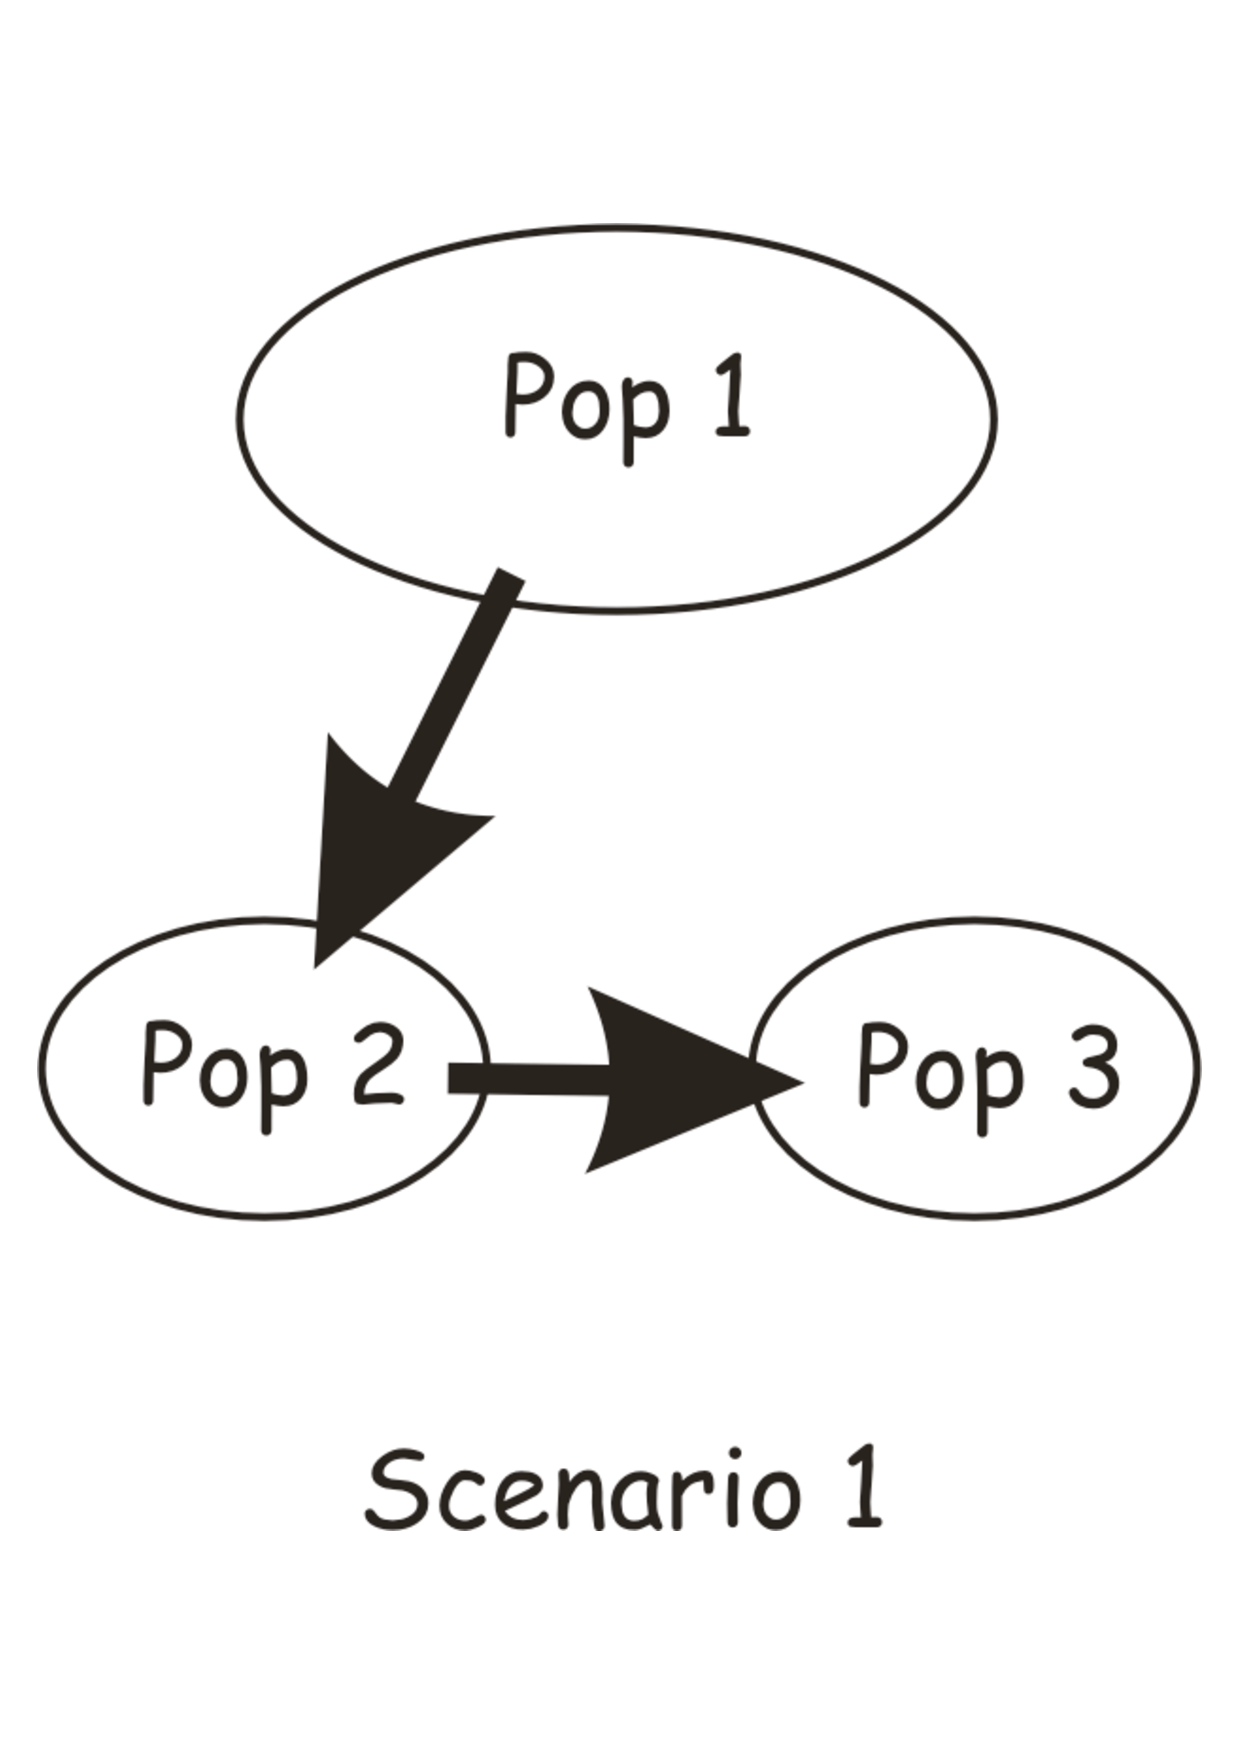
\includegraphics[scale=0.2]{scenario_invasion_1.pdf} &
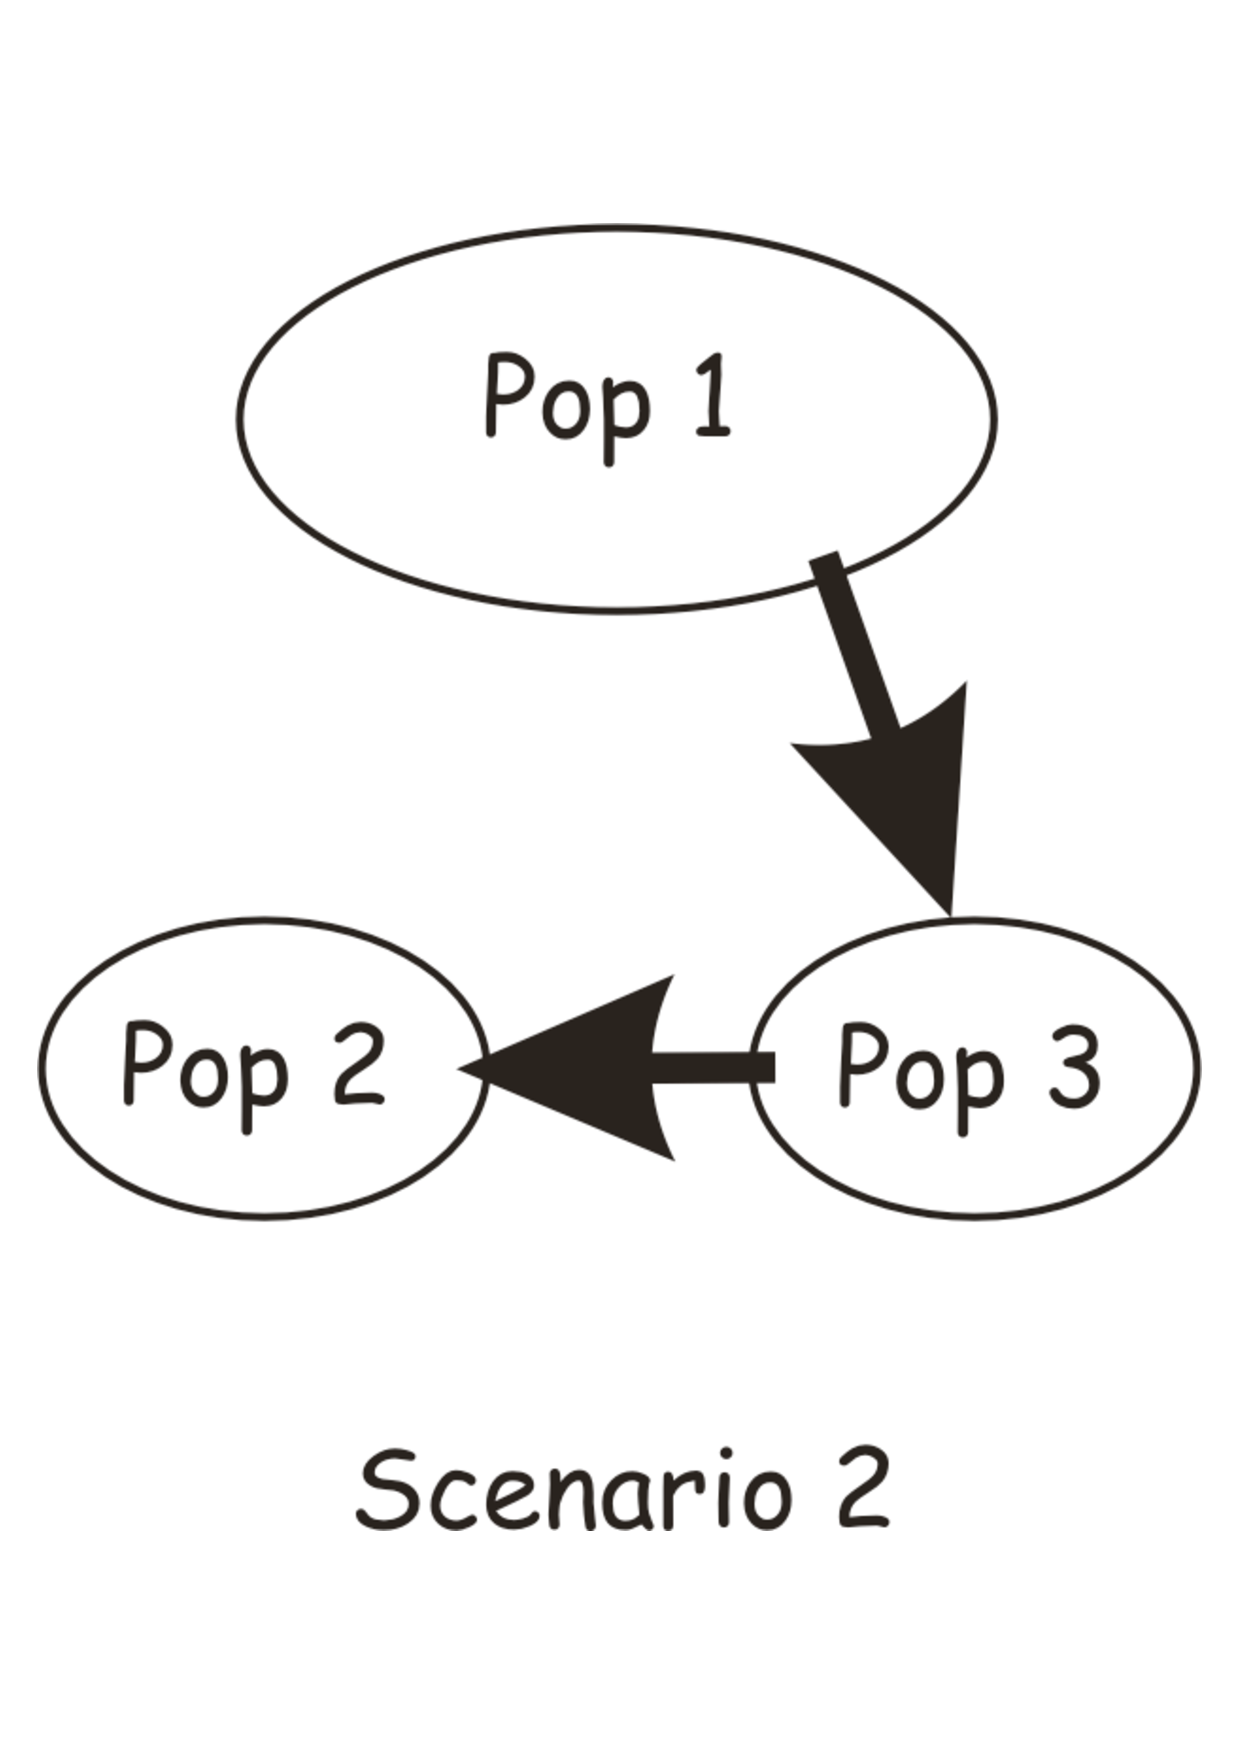
\includegraphics[scale=0.2]{scenario_invasion_2.pdf} &
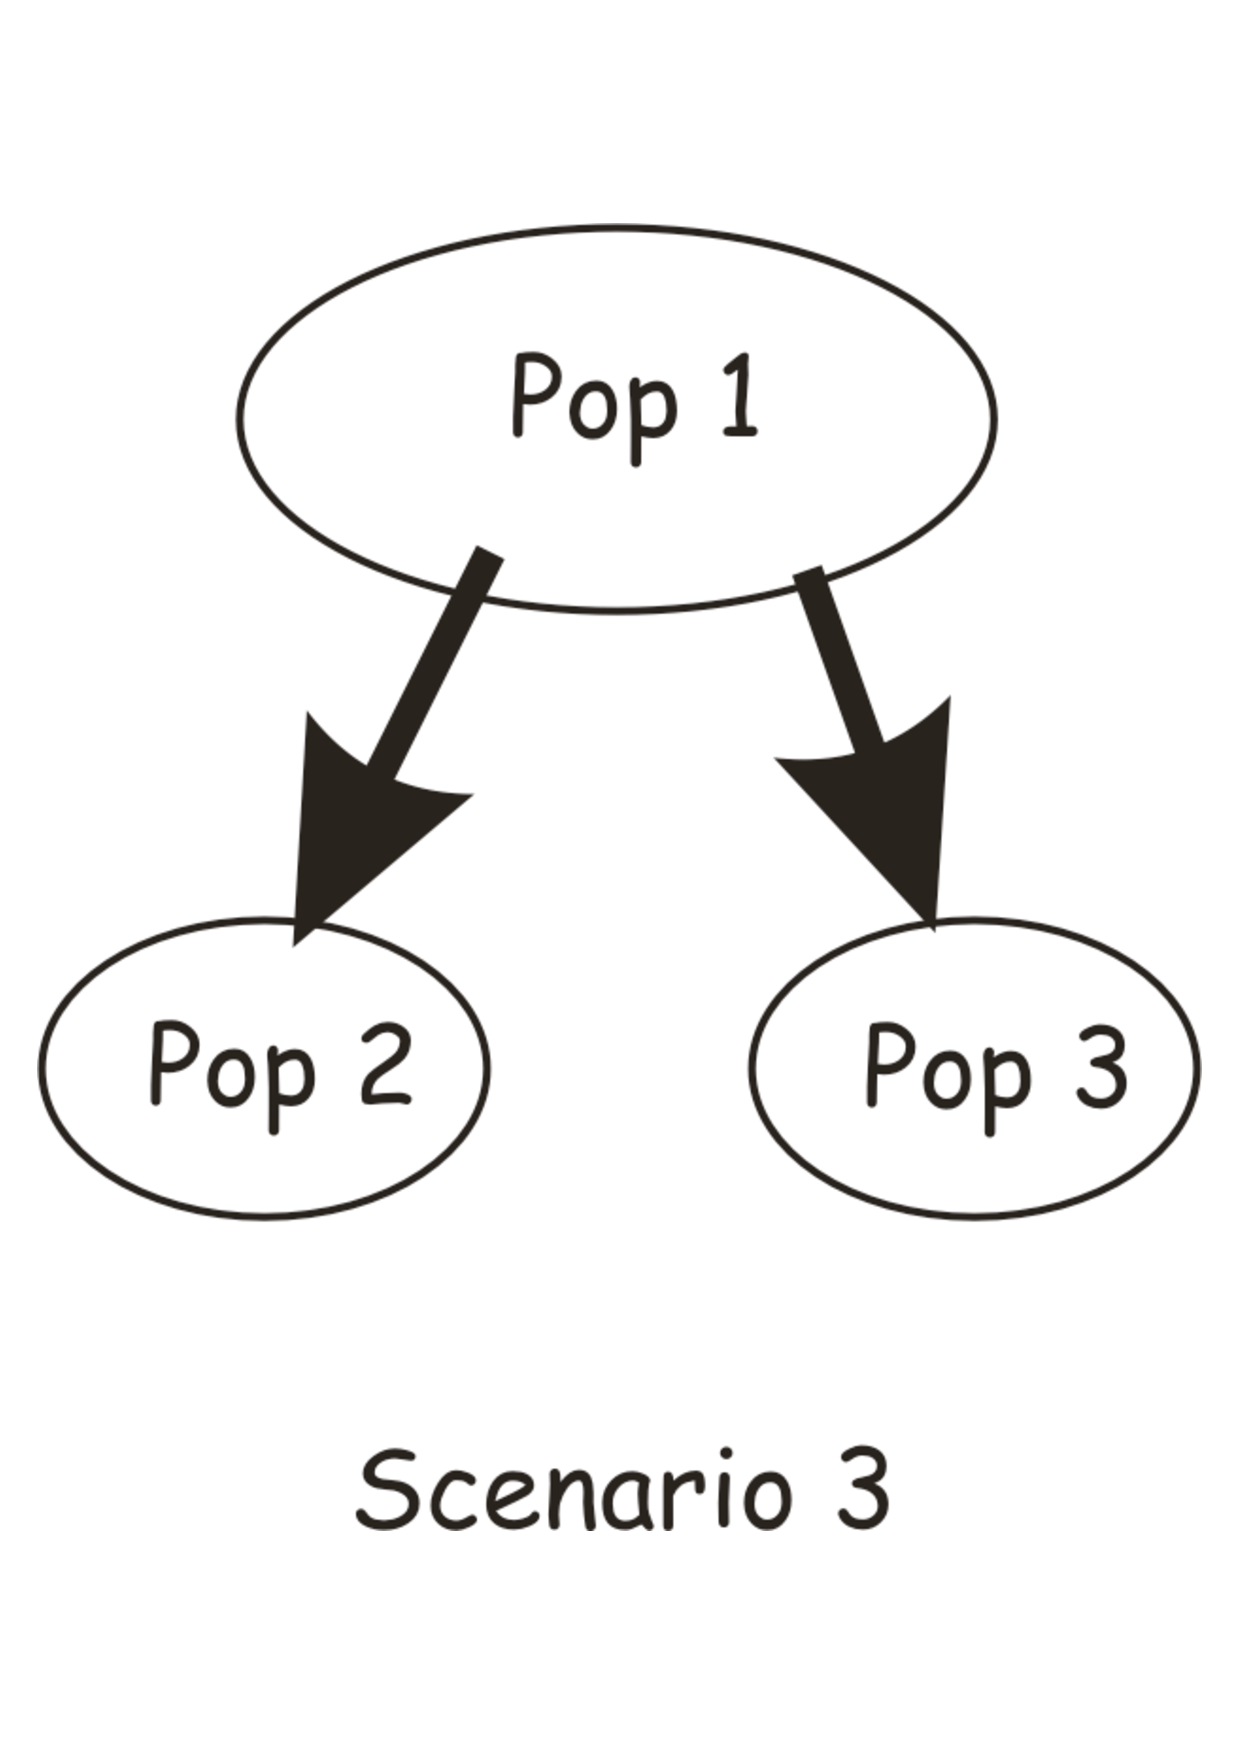
\includegraphics[scale=0.2]{scenario_invasion_3.pdf}
\end{tabular}
\end{center}
\end{figure}

The scenarios can be parameterized in the following way : we suppose that there is a common effective population size (say $N_s$) in the three populations. This (stable) population size on the two islands has been reached after a few generations ($db$) during which the effective size was much lower (only a few migrants reached the islands which corresponds to a transitory bottleneck). Let $N_2$ and $N_3$ be these bottleneck population sizes for population 2 and 3 respectively.
We suppose that sample sizes are 25 diploid individuals per population, each individual having been genotyped at 10 autosomal microsatellite loci, 5 autosomal sequence loci and 1 mitochondrial sequence locus. Microsatellite loci are assumed to follow the SMM mutation model, each locus mutation rate drawn from a Gamma distribution (mean=mean mutation rate and shape=2). Autosomal sequence loci are all assumed to be 1000 nucleotide long and to follow the Kimura 2 parameter model. The number of constant sites is set to 10\% and the shape of the Gamma distribution for the mutation rate along the 1000 sites is set to 2. We also apply the same settings to the mitochondrial sequence locus. In our example, the sample of population 1 has been collected two generations after sampling population 2 and one generation before sampling population 3.\\


To provide an overview of program possibilities, we will go through the following steps :
\begin{enumerate}
\item simulate a data set  from scenario 1 with known values of parameters (note that biologists working on a real dataset do not need to go through this step),
\item using this simulated data set as a test data set compare scenarios 1, 2 and 3 to evaluate if there is one that fits better the data (i.e. that has a much higher posterior probability),
\item evaluate the level of confidence in the choice of the best supported scenario by estimating type I and II errors.  For that purpose, we will use test data files simulated with parameter values drawn from the same prior distributions as those used to build the reference table file under the scenario with highest posterior probability,
\item perform an ABC estimation of parameter values under the scenario with the highest posterior probability,
\item compute bias and mean square errors for parameter estimation. Here again, we will use test data files simulated as in step 3,
\item check that  data sets simulated with parameters drawn from the posterior distribution and the best supported scenario provide summary statistics that are close to those the original (simulated) test data set obtained at step 1 (Model checking).
\end{enumerate}

\subsection{Simulate a data set}

When the program is launched (e.g. by clicking on the program icon), the following screen appears. Click the lower right button marked \fbox{\textsf{Simulate data sets}}.

%\begin{figure}[h]
%\begin{center}
%\includegraphics[scale=0.5]{ss5png/screen1.png}
%\end{center}
%\end{figure}

The following screen appears which will be used to define the scenario and the parameter values :

%\begin{figure}[h]
%\begin{center}
%\includegraphics[scale=0.5]{ss5png/screen2.png}
%\end{center}
%\end{figure}

\clearpage
The first step is to edit the scenario in the scenario edit windows as shown below :

%\begin{figure}[h]
%\begin{center}
%\includegraphics[scale=0.4]{ss5png/screen3.png}
%\end{center}
%\end{figure}


Clicking on  \fbox{\textsf{Check scenario}} will allow the program to make some checks on the logic of the scenario and if all seems OK, a graphical version of the scenario will be displayed \footnote{In case the scenario is too complex, the program may be unable to provide a graphic representation. In the latter case, the following message will appear on the screen : \emph{Scenario x seems OK. But the current version of DIYABC is unable to provide a valid graphic representation. Sorry for the inconvenience...}}:

%\begin{figure}[h]
%\begin{center}
%\includegraphics[scale=0.4]{ss5png/screen4.png}
%\end{center}
%\end{figure}

Clicking on the \fbox{\textsf{OK}} button allows to go back to the previous screen. Before exiting this screen, you can also print and/or save the graphic representations of scenarios (click on \fbox{\textsf{PRINT}} and/or \fbox{\textsf{SAVE}}).
\clearpage
First click on \fbox{\textsf{Define sample sizes}} and if necessary edit the default values which are 50 individuals per sample. Here, we set all three sample sizes to 25 individuals.

%\begin{figure}[h]
%\begin{center}
%\includegraphics[scale=0.4]{ss5png/screen5.png}
%\end{center}
%\end{figure}

Then Click on \fbox{\textsf{Choose parameter values}} to set the values of the 6 demographic parameters : \texttt{Ns}, \texttt{N2}, \texttt{N3}, \texttt{db}, \texttt{t1} and  \texttt{t2}. Sample sizes (\texttt{Ns}, \texttt{N2}, \texttt{N3}) and times (\texttt{db}, \texttt{t1} and  \texttt{t2}) are measured in number of individuals and generations, respectively.

%\begin{figure}[h]
%\begin{center}
%\includegraphics[scale=0.4]{ss5png/screen6.png}
%\end{center}
%\end{figure}

Once this is done, we go to the next screen by clicking the  \fbox{$>>$} (next) button. This screen is used to set the number of loci for each possible category. According to what we have decided before, we set the number of autosomal diploid loci to 10, the number of autosomal sequence loci to 5, the number of mitochondrial sequences to 1 and keep all other categories to zero.\\
\newpage
 We get the following screen.

%\begin{figure}[h]
%\begin{center}
%\includegraphics[scale=0.4]{ss5png/screen7.png}
%\end{center}
%\end{figure}

This screen has three red lights, one for each category of loci that requires a mutation model to be defined. This is performed by clicking on the corresponding button marked \fbox{\textsf{Define mutation model}}. For autosomal diploid loci, we get the following screen.

%\begin{figure}[h]
%\begin{center}
%\includegraphics[scale=0.4]{ss5png/screen8.png}
%\end{center}
%\end{figure}



We choose the SMM model, meaning we set the mean coefficient P and the corresponding shape of the to Gamma to 0 (third and fourth edit windows from top), we exclude Single nucleotide indel mutations (Mean SNI rate and Shape of the Gamma set to 0) and keep the default values for mean mutation rate and for the shape of the Gamma distribution for individual loci mutation rates as shown on screen of top of next page. We also keep default values for locus names, motif sizes and allele ranges.\\
It is worth stressing here that it is difficult to directly infer the range of microsatellite loci from a real data set, as the latter usually only includes a subset of populations of a single species. A value of 30 to 60 continuous allelic states is traditionally chosen in simulation studies based on microsatellite data. One of us (AE) recently made a meta-analysis on a large number of microsatellite loci and a large number of species (i.e. more than 100 species) which has shown that, although a large variance exists among loci and species, the mean allele size range (over all loci and over all species) was close to 40 continuous allelic states (data/results not shown). Therefore we have chosen the later value as default value. A larger allele size range within the real data set is automatically detected by DIYABC which provides a warning message to the user in this case. It is worth noting that results are usually robust to assumptions on allele size constraints (30 to 60 continuous allelic states; e.g. Pascual et al. 2007).
Finally, we would like to stress the fact that the number of alleles and the allele size range at a locus are two different features of a locus. For instance one can have a locus for which the observed allele size range in the genotyped populations (defined as (size\_max - size\_min)/size of repeat unit) is say 30, whereas the total number of observed alleles is substantially lower.\\

We get the following screen :


%\begin{figure}[h]
%\begin{center}
%\includegraphics[scale=0.4]{ss5png/screen8a.png}
%\end{center}
%\end{figure}

We go back to the previous "Genetic data" screen (click on \fbox{$OK$}) and proceed to the definition of the mutation model of autosomal sequence loci in the same way. Note that the red light for autosomal diploid microsatellites has turned green.

%\begin{figure}[h]
%\begin{center}
%\includegraphics[scale=0.4]{ss5png/screen8b.png}
%\end{center}
%\end{figure}

Clicking on the \fbox{\textsf{Define mutation model}} of autosomal diploid sequence loci leads to the following screen (top of next page).\\
 We keep all default values includingt that of the mean mutation rate (5E-9). The default mutation model is the Kimura 2 parameters, with 10\% of invariant sites and a shape of the Gamma equal to 2. Default sequence length is 1000 nucleotides and all four nucleotides are in equal frequencies. Finally, the mean kappa coefficient (transition/transversion) is set to 10 by default.

\newpage

%\begin{figure}[h]
%\begin{center}
%\includegraphics[scale=0.4]{ss5png/screen8c.png}
%\end{center}
%\end{figure}

Back to the "Genetic data" screen (click on \fbox{$OK$}), we define the mutation model of the mitochondrial sequence in the same way. As for autosomal sequences, we keep all default values including the mean mutation rate set to 5E-8 for mitochondrial DNA sequences \citep{HL2008}. However, since there is a single locus, we set the two shapes of the Gamma distribution (for the mutation rate and the kappa coefficient)  to 0 since we want its parameters identical to the mean values.

%\begin{figure}[h]
%\begin{center}
%\includegraphics[scale=0.4]{ss5png/screen8e.png}
%\end{center}
%\end{figure}

When going back to the "Genetic data", we note that all red lights have turned green (see top of next page), meaning that the program has enough information to proceed to the next step. Naturally, if we need to check or to change any setting concerning loci, it is still time to do so (just click again on the corresponding \fbox{\textsf{Define mutation model}} button).\\

\newpage

%\begin{figure}[h]
%\begin{center}
%\includegraphics[scale=0.4]{ss5png/screen8f.png}
%\end{center}
%\end{figure}

When everything seems OK, click on the  \fbox{$>>$} (next) button. The following screen appears :

%\begin{figure}[h]
%\begin{center}
%\includegraphics[scale=0.4]{ss5png/screen9.png}
%\end{center}
%\end{figure}

In this screen, we can tell how many datafiles we need, give them a name, tell where to save them on the computer. We can also provide a sex ratio for the species (useful in case there are non autosomal loci as in this example) and complete the title of the dataset(s) if necessary.\\

We keep all default values and just click on the \fbox{\textsf{START}} button. The progressbar at the bottom indicates the progression which should be almost instantaneous with a single data file produced.

\newpage

%\begin{figure}[h]
%\begin{center}
%\includegraphics[scale=0.5]{ss5png/screen9b.png}
%\end{center}
%\end{figure}

Once the program has simulated the required datafile(s) (indicated by the progressbar), we quit the program by clicking on the \fbox{\textsf{EXIT}}
button.\\


 In case there had been X-linked or Y-linked loci, the following screen would have appeared to let the user indicate the number of individuals of each sex within each population sample. Note that :
 \begin{enumerate}
 \item The total of males and females can be different from the value entered on the "Set historical models" screen (p19). Were it the case, the sum of males and females entered on the screen below is the one used by the program.
 \item The number of males and females provided in the screen below is independent of the species sex ratio provided in the previous screen. The former relates to the samples and the latter to the species.
 \end{enumerate}

%\begin{figure}[h]
%\begin{center}
%\includegraphics[scale=0.5]{ss5png/screen10.png}
%\end{center}
%\end{figure}

Using a text editor, we can have a look to this simulated data file (next page).

\newpage

%\begin{figure}[h]
%\begin{center}
%\includegraphics[scale=0.5]{ss5png/screen11.png}
%\end{center}
%\end{figure}

The file is in Genepop format, but with some additional features.
\begin{enumerate}
\item In the title line appears the sex ratio noted between \textsf{$<$} and \textsf{$>$} under the form \textsf{$<NM=1.00NF>$}. Since the title is generally only copied, this addition should not interfere with other programs using  Genepop datafiles. Also if there is no such sex ratio addition, DIYABC will consider by default that NM=NF.
\item After the locus name, there is an indication for the category of the locus which is $<A>$ for autosomal diploid loci, $<H>$ for autosomal haploid loci, $<X>$ for X-linked (or haplo-diploid) loci, $<Y>$ for Y-linked loci and $<M>$ for mitochondrial loci. If no category is noted, DIYABC will consider the locus as autosomal diploid or autosomal haploid depending on the corresponding genotype of the first typed individual.
\item Genotypes of microsatellite loci are noted with six digit numbers (e.g. 190188) if diploid and by three digit numbers (e.g. 190) if haploid.
\item Sequence locus are noted between  \textsf{$<$} and \textsf{$>$} . In addition each sequence allele is noted between brackets. For instance, a haploid sequence locus  will be noted $<[$GTCTA$]>$ and a diploid sequence locus $<[$GTCTA$][$GTCTT$]>$.
\item Missing microsatellite genotypes are noted \textsf{000} if haploid or \textsf{000000} if diploid.
\item Missing sequence genotypes are noted $<[]>$ if haploid or $<[][]>$ if diploid.
\end{enumerate}

Note that all the above additions have been made to keep as much as possible compatibility with the usual Genepop format.\\


Once we dispose of a datafile (\texttt{gp\_001.txt}), we can go to the next step. Note that this would be the first step if we had an observed data file. Whatever the analysis we want to perform, we will need a \emph{reference table}, i.e. a table in which are written parameter values and summary statistics of simulated data sets. In the next section, we explain how to build such a table with DIYABC.


\newpage
\subsection{Build a reference table}
Launch the program and click on the bottom left button marked \fbox{\textsf{Perform an ABC analysis}}.

%\begin{figure}[h]
%\begin{center}
%\includegraphics[scale=0.4]{ss5png/screen1.png}
%\end{center}
%\end{figure}


 The following screen appears :

%\begin{figure}[h]
%\begin{center}
%\includegraphics[scale=0.4]{ss5png/screen12.png}
%\end{center}
%\end{figure}


Clicking on the \fbox{\textsf{Data file}} button allows to choose a data set through the usual Windows dialog :

%\begin{figure}[h]
%\begin{center}
%\includegraphics[scale=0.4]{ss5png/screen12a.png}
%\end{center}
%\end{figure}

We type the name of the data file that was just simulated before or click on it in the list. The program
looks for any reference table made for this particular data set and that would be present in the same directory.\\
\newpage
 Since there is no such reference table, the screen will look like this :

%\begin{figure}[h]
%\begin{center}
%\includegraphics[scale=0.35]{ss5png/screen13.png}
%\end{center}
%\end{figure}

The program suggests a default name for the reference table. We can leave it or change it by typing a new name in the edit window. We then exit the screen (click on \fbox{\textsf{OK}}) and the "Data and analysis" screen reappears with information on the data file (number of populations, individuals and loci). It also says what we need to do next to build the reference table.

%\begin{figure}[h]
%\begin{center}
%\includegraphics[scale=0.35]{ss5png/screen14.png}
%\end{center}
%\end{figure}
We go to the next screen which is used to define the scenario and the prior distributions of parameters  by clicking on the \fbox{$>>$} button.


\newpage
We get the following screen :
%\begin{figure}[h]
%\begin{center}
%\includegraphics[scale=0.45]{ss5png/screen15.png}
%\end{center}
%\end{figure}

We edit a first scenario, which is the same as in the first subsection.
%\begin{figure}[h]
%\begin{center}
%\includegraphics[scale=0.45]{ss5png/screen16.png}
%\end{center}
%\end{figure}

Then by clicking on the  \fbox{\textsf{Add scenario}} button, we open a second scenario edit windows.

\newpage
We fill in this second scenario, swapping between populations 2 and 3 (cf scenario 2, page 10). Note that the addition of the second scenario automatically opened a panel to set prior probabilities on scenarios.

%\begin{figure}[h]
%\begin{center}
%\includegraphics[scale=0.45]{ss5png/screen17.png}
%\end{center}
%\end{figure}

Eventually, we add a third scenario (cf scenario 3, page 10) corresponding to independent invasions of the two islands.

%\begin{figure}[h]
%\begin{center}
%\includegraphics[scale=0.45]{ss5png/screen18.png}
%\end{center}
%\end{figure}

In this third scenario, we have renamed the times \texttt{t1} and \texttt{t2} to \texttt{t3} and \texttt{t4}, because in the first two scenarios, we have to set the condition \texttt{t2} $>$ \texttt{t1} to make these scenarios possible whereas no such condition is necessary for the third scenario, although we could have chosen to do so. The condition on \texttt{t1} and \texttt{t2} will have an impact on their respective prior distributions that we do not desire for \texttt{t3} and \texttt{t4}.

\newpage
Clicking on the  \fbox{\textsf{Check scenario}} button, we can visualize the three scenarios.

%\begin{figure}[h]
%\begin{center}
%\includegraphics[scale=0.45]{ss5png/screen19.png}
%\end{center}
%\end{figure}

Then by clicking on the  \fbox{\textsf{Define priors}} button, we can set prior distributions by editing the panels corresponding to each parameters. The program takes as a parameter any character string other than the keywords \texttt{sample, merge, split} and \texttt{varNe} appearing in the scenario windows. On the following screenshot, we can see priors only for the first four scenario parameters. The other parameters can be seen and their windows edited either by using the scrollbar on the right or by enlarging the screen as in any Windows application.

%\begin{figure}[h]
%\begin{center}
%\includegraphics[scale=0.45]{ss5png/screen20.png}
%\end{center}
%\end{figure}

Choose the distribution density (Uniform, Loguniform, Normal or Lognormal) by clicking into the corrresponding  checkbox and edit the default values if necessary. Clicking on a  \fbox{\textsf{set condition}} button allows to set a relationship between values for two parameters of the same category (effective size, time or admixture rate). Here, we want \texttt{t2} to always be greater than \texttt{t1}, so we click on the \texttt{set condition} button on the \texttt{t2} panel. This opens the following windows (next page) :

\newpage

%\begin{figure}[h]
%\begin{center}
%\includegraphics[scale=0.45]{ss5png/screen21.png}
%\end{center}
%\end{figure}

Here, we will keep uniform distributions for all parameters. We will set intervals [10000,1000000] for  \texttt{Ns} and [1,100] for  \texttt{N2},  \texttt{N3},  \texttt{t1}, \texttt{t2}, \texttt{t3} and  \texttt{t4}. Eventually, we set
the minimum and maximum values of \texttt{db}  to 5. It results that \texttt{db} will be taken as a constant. It will disappear from the list of parameters in the following analyses. Note that time parameters are scenario specific and that only the three population sizes are common to all three scenarios. Note also that in this screenshot, all parameters are now visible (the screen has been extended vertically).

%\begin{figure}[h]
%\begin{center}
%\includegraphics[scale=0.45]{ss5png/screen22.png}
%\end{center}
%\end{figure}

By imposing a condition on parameters ($\texttt{t2}>\texttt{t1}$), we were offered a choice between two options. The default option is that successive sets of parameter values are drawn at random until one set fulfills all imposed conditions. The other option is to draw a single set. If it fulfills all conditions, then the set is used to produce a data set that is recorded in the reference table. If it does not, no data set is simulated and nothing is added to the reference table. Here we leave the default option.
\\
We can now leave this screen and inform the next one by clicking on the \fbox{\textsf{$>>$}} next button. \\
\newpage
The following screen appears :

%\begin{figure}[h]
%\begin{center}
%\includegraphics[scale=0.45]{ss5png/screen23.png}
%\end{center}
%\end{figure}

The above screen tells us that we need to define the mutation model for 3 categories of loci (autosomal diploid microsatellites, autosomal diploid DNA sequence loci and mitochondrial DNA sequence locus).
We start clicking on the \fbox{\textsf{Define mutation model}} of the 10 microsatellite loci and obtain the following screen.

%\begin{figure}[h]
%\begin{center}
%\includegraphics[scale=0.45]{ss5png/screen24.png}
%\end{center}
%\end{figure}

We keep all default values except for the SNI mutation rate that we set to 0 (minimum and maximum of the mean rate to fix the mean rate to 0 and shape of the Gamma distribution to have all loci rates identical to the mean). Note that leaving default values for coefficient P  means that in the reference table, we choose a GSM model. In this particular case, we know that the datafile has been simulated with the SMM, but with observed data files, we do not know and we (almost surely) will not choose the true mutation model. So let us see whether choosing an erroneous model (GSM instead of SMM) will lead to some erroneous conclusions in this case.

\newpage
%\begin{figure}[h]
%\begin{center}
%\includegraphics[scale=0.45]{ss5png/screen25.png}
%\end{center}
%\end{figure}

When we are happy with the content of this screen, we click on the  \fbox{\textsf{OK}} to go back to the previous screen in which the corresponding red light has turned green. We do the same for the mutation model of the two sequence loci categories (next two screens).

%\begin{figure}[h]
%\begin{center}
%\includegraphics[scale=0.45]{ss5png/screen26.png}
%\end{center}
%\end{figure}

In the above screen, we keep all default values. In the next screen (next page), we do the same except for the individual locus so that the locus mutation rate has the same range of values as the mean (this is our choice, we could as well leave the default values).
\newpage

%\begin{figure}[h]
%\begin{center}
%\includegraphics[scale=0.45]{ss5png/screen27.png}
%\end{center}
%\end{figure}


After setting the mutation models, the "Genetic data" screen now looks like this :

%\begin{figure}[h]
%\begin{center}
%\includegraphics[scale=0.45]{ss5png/screen28.png}
%\end{center}
%\end{figure}

We have still to define the summary statistics for each category of loci (buttons with red lights).\\

Let define first the summary statistics of the 10 microsatellite  loci (click on the corresponding  \fbox{\textsf{Define summary statistics}} button). The following screen (next page) appears.

%\begin{figure}[h]
%\begin{center}
%\includegraphics[scale=0.45]{ss5png/screen29.png}
%\end{center}
%\end{figure}

\newpage
We choose all one sample summary statistics, as well as all Fst and Classification indices by clicking the corresponding checkboxes.
%\begin{figure}[h]
%\begin{center}
%\includegraphics[scale=0.45]{ss5png/screen30.png}
%\end{center}
%\end{figure}

Then we exit the screen ( \fbox{\textsf{OK}}) and we define the summary statistics of the 5 autosomal sequences with the following screen (next page).

\newpage

%\begin{figure}[h]
%\begin{center}
%\includegraphics[scale=0.4]{ss5png/screen31.png}
%\end{center}
%\end{figure}

We choose the first three one sample summary statistics as well as the two means (between and within) of pairwise differences (two sample summary statistics).

%\begin{figure}[h]
%\begin{center}
%\includegraphics[scale=0.4]{ss5png/screen32.png}
%\end{center}
%\end{figure}

Eventually, we define the summary statistics for the mitochondrial DNA sequence in the same way (screens not shown).\\

When all desired summary statistics have been selected for the three categories of loci, all lights of the "Genetic data" screen have turn green (shown next page).

\newpage

%\begin{figure}[h]
%\begin{center}
%\includegraphics[scale=0.4]{ss5png/screen_geneticdata.png}
%\end{center}
%\end{figure}

We can now click on the next ( \fbox{\textsf{$>>$}}) button and get the following screen.

%\begin{figure}[h]
%\begin{center}
%\includegraphics[scale=0.4]{ss5png/screen33.png}
%\end{center}
%\end{figure}



The next screen  corresponds to the building of the reference table. The default value for the number of newly simulated data is 1,000,000 per scenario, i.e. 3,000,000 in our three scenario case and the reference table is empty.
We set the number of simulated data sets to e.g. 1,500,000, which corresponds to 500,000 datasets per scenario,
% \footnote{The current models have each 6 true parameters (3 effective sizes, 2 divergence times and the mean mutation rate). They define a space (the parameter space) that needs to be explored thoroughly enough.  There is no precise rule to compute the number of simulated data sets required in any reference table. However, it is usually considered reasonable to take it of the order of 10$^p$ ($p$=number of parameters), which would put it here at 10$^6$ for each scenario.}
and click on the \fbox{\textsf{START}} button.

\newpage

 We can follow the progression of simulations on the progress bar and on the label at the center of the screen. The program also provides the current size of the reference table file (updated every 10000 simulated data sets) as well as an estimation of the remaining computation time. Note that during data simulation, only the \fbox{\textsf{STOP}} button is active. It has to be clicked on before any other control.


%\begin{figure}[h]
%\begin{center}
%\includegraphics[scale=0.45]{ss5png/screen34.png}
%\end{center}
%\end{figure}


When the 1,500,000 data sets have been simulated (this took about 15 hours on a desktop equipped with a  X5550 Intel bi-processor), the screen disappears and is replaced by the following Data and analysis screen.



%\begin{figure}[h]
%\begin{center}
%\includegraphics[scale=0.45]{ss5png/screen35.png}
%\end{center}
%\end{figure}

This screen tells us that a reference table named \texttt{gp\_001.reftable} is now available and that we can proceed to any other step of the ABC analysis.

\newpage

If for any reason,  we want to look at the content of the reference table \texttt{gps\_001.reftable}, we need to convert the file format from binary to text. We need to go back to the previous screen by choosing the (default) option "Append new simulations to the reference table" and clicking three times on the  \fbox{\textsf{$>>$}} button. We then click on the option \texttt{Export reference table} in the \texttt{Options} menu :

% \begin{figure}[h]
%\begin{center}
%\includegraphics[scale=0.8]{ss5png/screen36.png}
%\end{center}
%\end{figure}

This opens the following window. If there are more than one scenario, the user can choose between two options : (i) either exporting the reference table as a whole or  (ii) splitting the reference table putting simulated data sets of different scenarios into separate text files. Note that these converted text files cannot be used by DIYABC. The names of the text files are automatically built from that of the binary file.

%\begin{figure}[h]
%\begin{center}
%\includegraphics[scale=0.5]{ss5png/screen37.png}
%\end{center}
%\end{figure}

Click on \fbox{\textsf{START}} to begin the conversion. The window will automatically close at the end of the conversion. For a large reference table, this export process can take some time. A progress bar indicates what proportion of the file transfer has been achieved. Note that it is possible to exit the window without completing the transfer by clicking on the \fbox{\textsf{OK}} button. In this case, only the header and a fraction of the reference table will appear in the output file.

%\begin{figure}[h]
%\begin{center}
%\includegraphics[scale=0.5]{ss5png/screen38.png}
%\end{center}
%\end{figure}


Once a sufficiently large reference table has been built, we can proceed to the estimation part of the ABC analysis, the latter using the binary file \texttt{gps\_001.reftable}. To do so, click on the option \texttt{Data and analysis} of the \texttt{Options} menu (see top of page). You can also quit the program (same menu, \texttt{Quit} option).

\newpage
\subsection{Pre-evaluation of scenario-prior combinations}

If we have quitted the program, we launch it again and select the top button \fbox{\textsf{Perform an ABC analysis}}. On the following screen, we click on the \fbox{\textsf{Data file}} button and select the data file \texttt{gps\_001.txt }. The program finds now a reference table made for this data file (screen below). If we did not exit the program and used the  \texttt{Data and analysis}  option instead (see bottom of p28), the screen below is skipped and the default option is taken automatically.

%\begin{figure}[h]
%\begin{center}
%\includegraphics[scale=0.45]{ss5png/screen39.png}
%\end{center}
%\end{figure}

We take the default option and exit the window (click on \fbox{\textsf{OK}} button). We are back to the Data and analysis screen (screenshot below which is the same as that shown on page 38).

%\begin{figure}[h]
%\begin{center}
%\includegraphics[scale=0.45]{ss5png/screen40.png}
%\end{center}
%\end{figure}

In this example, the "observed data file" has been actually simulated. Hence we know the true scenario and the true values of the parameters. However, this is not generally the case with biological data. It is therefore a wise step before any further treatment to check whether the combination of scenario(s) and prior distributions of their parameters can indeed produce data sets that are similar enough to the observed data set. This can be achieved through the option "Pre-evaluate scenario-prior combinations" at the bottom of the "Data and Analysis" screen. This option is designed to detect models unable to explain the data. This can happen with mis-specified  evolutionary scenario(s) or  prior distribution(s).

\newpage
Clicking on the next (\fbox{\textsf{$>>$}}) button leads to the following screen :

%\begin{figure}[h]
%\begin{center}
%\includegraphics[scale=0.4]{ss5png/screen71.png}
%\end{center}
%\end{figure}

 There are two options proposed to the user :
 \begin{enumerate}
 \item perform a principal component analysis (PCA) of the first (up to) 100,000 simulated data sets of the reference table in the space of summary statistics, and evaluate the position of the observed data set compared to simulated data sets,
 \item  locate each summary statistics of the observed data set among those of the simulated data sets.

\end{enumerate}

Let us click on the \fbox{\textsf{Perform PCA}}. A new windows opens where we can see the progression of computations and eventually a graph showing the first plane of the analysis (below).

%\begin{figure}[h]
%\begin{center}
%\includegraphics[scale=0.5]{ss5png/screen72.png}
%\end{center}
%\end{figure}

We can see that the observed data set (large yellow dot) is surrounded by many simulated data sets (small dots) indicating that our model is able to produce data sets similar to the observed one. Given that the observed data set has been actually simulated according to scenario 1 with parameter values included in the prior distribution support, this was of course expected. After closing this window (\fbox{\textsf{CLOSE}} button), we launch the second option by clicking on the \fbox{\textsf{Locate observed S.S. among simulated}} and get the following screen.

\newpage

%\begin{figure}[h]
%\begin{center}
%\includegraphics[scale=0.4]{ss5png/screen73.png}
%\end{center}
%\end{figure}

We observe that most observed summary statistics are well in the range of simulated ones. However, we see an increasing number of marginal summary statistics (noted by one, two or three stars when the observed S.S. is in the 5\%, 1\% or 0.1\% tails of distributions respectively) from scenario 1 to scenario 3. This can be seen as a first clue that scenario 1 is better supported than the other two scenarios. This result is however clearly insufficient to make any robust inference and further treatments are obviously needed (see next section).
\newpage
\subsection{Compare scenarios by computing their posterior probabilities}


We select the option to compare scenarios (bottom option : \emph{Compute posterior probabilities of scenarios}) and we click on the \fbox{\textsf{$>>$}} button three times until reaching the following screen (next page).


%\begin{figure}[h]
%\begin{center}
%\includegraphics[scale=0.45]{ss5png/screen41.png}
%\end{center}
%\end{figure}

This allows to compare any combination of at least two scenarios. If the reference table contains only two scenarios, this screen is skipped. We leave the default choice, i.e. all three scenarios, and click on the \fbox{\textsf{OK}} button. The following is now entirely visible.

%\begin{figure}[h]
%\begin{center}
%\includegraphics[scale=0.45]{ss5png/screen42.png}
%\end{center}
%\end{figure}

We can then choose the number of simulated data from the reference table that we want to keep for the analysis (must be $\leq$ the total number available in the reference table) and the number of selected data (i.e. simulated data closest to observed data) for the direct estimate and the logistic regression. We keep all simulated data and default values for the numbers of simulated data sets closest to observed, i.e. 500 for the Direct estimate approach and 15,000 (1\%  proportion) for logistic regression approach.The time spent for the logistic regression raises more or less linearly with the number of closest data sets, and quadratically with the number of scenarios (minus one) and with the number of summary statistics. With more than a very few scenarios (e.g.$>$5) and a rather large number of summary statistics (e.g. 50), the logistic regression computations can last hours. By default, the program performs 10 logistic regressions (in our example, with 1,500, 3,000, ...15,000 closest data sets) but this number can be reduced to 1 or even 0. Indeed, it can be useful in some cases to skip it to get a rough idea of the relative support of scenarios through the direct estimate only. One can then proceed to the logistic regression computations on the subset of scenarios with non null support under the direct estimate.

\newpage

Clicking on the \fbox{\textsf{Run computations}} button starts the computations and the progression is visible in a new window as shown below.

%\begin{figure}[h]
%\begin{center}
%\includegraphics[scale=0.5]{ss5png/screen43.png}
%\end{center}
%\end{figure}

At the end, this windows shows a log of all computations which can be saved in a log file ( \fbox{\textsf{Save log file}} button).

%\begin{figure}[h]
%\begin{center}
%\includegraphics[scale=0.5]{ss5png/screen44.png}
%\end{center}
%\end{figure}

We close the window by clicking on the  (\fbox{\textsf{Close window}} button), to get back to the previous window, in which are shown two graphs (screenshot on next page.\\
On the left, posterior probabilities of scenarios are simply the relative proportions of each scenario found in the selected closest data sets ("Direct estimate"), the number of the latter varying between 1\% and 100\%  of the number written in the edit windows (here 500). On the right, posterior probabilities of scenarios are obtained through a logistic regression, computed every 10\% (between 10 and 100\%) of the number of selected data sets.\\

\newpage

%\begin{figure}[h]
%\begin{center}
%\includegraphics[scale=0.5]{ss5png/screen45.png}
%\end{center}
%\end{figure}

 In this particular example, both approaches are congruent and show maximum support for the first (i.e. true) scenario. Such a clear output is far from being the rule when analyzing real data sets. In our experience, the logistic regression is generally more discriminant than the direct estimate \citep{C2008}. Also, the direct estimate is more sensitive to the number of closest simulated data sets than the logistic regression (clearly taking more and more simulated data sets, the direct estimate will converge towards  prior probabilities). However, with too low numbers of closest data sets, the logistic regression can be unstable and the default proportion of 1\% seems to be a threshold above which stable results are generally obtained \citep[see e.g.][]{G2010,L2010}.


 . Graphs can be printed (\fbox{\textsf{Print graphs}} button) and saved (\fbox{\textsf{Save graphs}} button) and numerical values can be saved (\fbox{\textsf{Save output}} button).\\
Below is a reproduction of the output file (obtained by clicking on the \fbox{\textsf{Save output}} button. The 95\% confidence limits for the direct approach are simply the 95\% bounds of a binomial proportion and should not be considered as those of the posterior probability of scenarios.  For the logistic approach on the contrary, the 95\% confidence interval is much more meaningful, at least for sample sizes that are small enough to justify a linear approximation of the logit of posterior probabilities \citep[see][]{C2008}.

%\begin{figure}[h]
%\begin{center}
%\includegraphics[scale=0.7]{ss5png/screen46.png}
%\end{center}
%\end{figure}

\newpage

 We can get a visual information on how data sets simulated under each scenario are close or not from the observed data set by running a PCA clicking on the button  \fbox{\textsf{Visualize PCA}}. In this PCA, the observations are the simulated data sets and the variables are the summary statistics. Once the analysis has been performed, the observed (the simulated pseudo-observed data set in our example) is added in the space of the analysis. Several options have been implemented for visualizing the results: choice of the principal components, choice of  the scenarios (individually or all together), number of points that are represented (see examples below). Output can also be printed or saved (the file name is composed of the title of the graph with the extension \texttt{bmp}, e.g. the graph of the third example will be saved with the name \texttt{gp\_001\_PCA\_1\_2\_20000.bmp})\\
 \begin{center}
 \textbf{Example 1} : All scenarios : principal components 1 and 2
 \end{center}
%\begin{figure}[h]
%\begin{center}
%\includegraphics[scale=0.35]{ss5png/screen47.png}
%\end{center}
%\end{figure}

 \begin{center}
 \textbf{Example 2} : Scenario 2 : principal components 1 and 5
 \end{center}
%\begin{figure}[h]
%\begin{center}
%\includegraphics[scale=0.35]{ss5png/screen48.png}
%\end{center}
%\end{figure}

Example 1 shows the data sets simulated with the three scenarios on the first plane of the analysis. One can see that the pseudo-observed data set has a rather marginal position compared to data sets simulated with scenario 3. Example 2 shows the same situation with the second scenario in another plane.

\newpage
\subsection{Estimate posterior distributions of parameters}

Restarting the program as in section 3.3, or going directly from last screen using the option "Data and analysis" of the "Options" menu, we reach the "Data and analysis" screen.We choose the second option "Estimate posterior distributions of parameters and model checking".

%\begin{figure}[h]
%\begin{center}
%\includegraphics[scale=0.4]{ss5png/screen49.png}
%\end{center}
%\end{figure}

Click on the \fbox{\textsf{$>>$}}  button until reaching the following screen :
%\begin{figure}[h]
%\begin{center}
%\includegraphics[scale=0.5]{ss5png/screen50.png}
%\end{center}
%\end{figure}

We can choose any combination of at least one scenario. If a single scenario is chosen, all its parameters will be estimated. If two or more scenarios are selected, only parameters that are common to all these scenarios will be estimated. In the current example, since scenario 1 is by far the most supported scenario (as seen in the previous section), we will restrict our choice to this single scenario.

\newpage
When exiting the previous screen (scenario choice), we get the following screen, which is similar to the one for running comparison of scenario. However, it offers two additional choices : "transformation of parameters" and "choice of parameters".\\
 Most generally, parameters take values on bounded intervals, with positive bounds. If no transformation is applied to parameters, it may happen that samples from the posterior distribution, obtained through local linear regressions, contain values outside the prior limits. It is therefore advisable to perform the regression on transformed parameter values and to backtransform them at the end. Let's use the \emph{logit} transformation (default choice), but the program allows also the \emph{log-tg} \citep{HS2005} or the simple \emph{log} transformation \citep{EB2004}, as well as no transformation at all
\footnote{$logit(x,a,b)=log(\frac{x-a}{b-x})$ and \emph{log-tg}$(x,a,b)=log(tg(\frac{x-a}{b-a}\frac{\pi}{2}))$ with $a$ and $b$ lower and upper bound of prior interval, respectively.}. Note that only the $logit$ and $log-tg$ transformations ensure that sampled values from the posterior distribution of parameters will be within prior limits.\\
Original parameters are effective population sizes, times, admixtures rates and mean mutation parameters ($\bar{\mu}$ and $\bar{P}$). However, in many instances, scaled parameters are easier to estimate (they are sometimes the only estimable parameters). So if the "composite" box is ticked, the program will estimate parameters $\theta  = N_e\mu$ and $\tau = t\mu$.
%\begin{figure}[h]
%\begin{center}
%\includegraphics[scale=0.45]{ss5png/screen51.png}
%\end{center}
%\end{figure}

Here, we will leave the two default options : \emph{logit} transformation and both \emph{original} and \emph{composite} parameters. We also note that the program has found 501,015 data sets simulated with scenario 1 in the reference table. We keep them all and leave the default 1\% (5,010) value for the number of selected data sets for the local linear regression. Then we launch computations by clicking on the \fbox{\textsf{Run}} button.

\newpage
A new window opens on top of the previous one. It shows the progression of computations.

%\begin{figure}[h]
%\begin{center}
%\includegraphics[scale=0.5]{ss5png/screen52.png}
%\end{center}
%\end{figure}

When the computations are over (\textsf{COMPUTATION TERMINATED} at the bottom of the window, screen below), we close this window (\fbox{\textsf{Close window}} button). The other button {\fbox{\textsf{Save log file}} can be used to save the content of the window (i.e. log file).

%\begin{figure}[h]
%\begin{center}
%\includegraphics[scale=0.5]{ss5png/screen53.png}
%\end{center}
%\end{figure}

\newpage

The underlying window reappears showing the posterior distributions of all original and composite parameters. The red and green lines show the prior and posterior distributions, respectively. In the title of each graph is also given a point estimate, which is the median of the posterior distribution.\\
Below each graph, there is a set of summary statistics of the posterior distribution of the parameter.


%\begin{figure}[h]
%\begin{center}
%\includegraphics[scale=0.5]{ss5png/screen54.png}
%\end{center}
%\end{figure}

The graphs shown on the screen can be printed (\fbox{\textsf{Print graphs}} button) or saved ( \fbox{\textsf{Save graphs}} button). If they are saved, they are automatically saved individually in bitmap format, with name taken as the title of each graph in wich \emph{space} and \emph{colon}  characters have been disgarded (e.g. \texttt{ParameterNs[median=2.45E+003].bmp}).\\
The summary statistics can be printed (\fbox{\textsf{Print output}} button) or saved ( \fbox{\textsf{Save output}} button). \\

Below is the output file obtained by clicking on the \fbox{\textsf{Print output}} or the \fbox{\textsf{Save output}} button.
%\begin{figure}[h]
%\begin{center}
%\includegraphics[scale=0.5]{ss5png/screen55.png}
%\end{center}
%\end{figure}

\newpage

Clicking on the \fbox{\textsf{Save [phi*]}} button allows to save the parameter values used to compute the posterior densities of each parameter \citep[after correction by the weighted linear regression;][]{B2008} . This can be useful if one wants to perform additional computations or to draw more graphs, e.g. using R \citep{IG1996}. The upper left part of the phi* file looks like this :

%\begin{figure}[h]
%\begin{center}
%\includegraphics[scale=0.7]{ss5png/screen56.png}
%\caption{Upper left part of a phi* file providing the corrected values of parameters from the 5,010 closest data sets, sorted by ascending distances. }
%\end{center}
%\end{figure}


\newpage
\subsection{Model checking}
In Bayesian analysis assessing the �goodness-of-fit� of a model (here a scenario) is termed model checking. Following Gelman et al. (1995; pp 159-163), if a model fits then replicated data generated under the model should look similar to observed data. To put it another way, the observed data should look plausible under the posterior predictive distribution. This is really a self-consistency check: an observed discrepancy can be due to model misfit (demographic and/or marker models) or chance. We implemented an option in DIYABC to measure the discrepancy between model and real data by considering various sets of test quantities. These test quantities can be chosen among the large set of ABC summary statistics proposed in DIYABC. For details and examples regarding the choice of summary statistics as test quantities, see \citet{C2010}.\\
In the previous screen ("ABC parameter estimation"), let us click on the \fbox{\textsf{Model checking}} button. The following screen appears :

%\begin{figure}[h]
%\begin{center}
%\includegraphics[scale=0.5]{ss5png/screen57.png}
%\end{center}
%\end{figure}

We click on the only enabled button (\fbox{\textsf{SIMULATE FROM PHISTAR}}. The following screen appears in which we can choose summary statistics for first category of loci (autosomal diploid microsatellites)

%\begin{figure}[h]
%\begin{center}
%\includegraphics[scale=0.5]{ss5png/screen58.png}
%\end{center}
%\end{figure}

Here, we choose to keep all one sample summary statistics and to choose all available two sample summary statistics that have not been computed in the reference table (screen on next page):

%\begin{figure}[h]
%\begin{center}
%\includegraphics[scale=0.5]{ss5png/screen59.png}
%\end{center}
%\end{figure}

\newpage
Clicking on the \fbox{\textsf{OK}} button, we get the screen allowing to choose summary statistics for the next  category of loci (DNA sequence loci). It is not shown here because we just keep the suggested summary statistics (the same as in the reference table), so that we just clicked on the  \fbox{\textsf{OK}} button. We do the same with the last category (MtDNA locus). When this has been done, the following screen is shown.

%\begin{figure}[h]
%\begin{center}
%\includegraphics[scale=0.35]{ss5png/screen60.png}
%\end{center}
%\end{figure}

We keep the default value for the number of new data sets(1000) and launch simulation by clicking on the \fbox{\textsf{Run computation}}. First the program counts how many of the 5010 phistars comply with the conditions set on the parameters. Because of the "correction" by the local linear regression, some phistars are such that they do not observe the conditions. We have to extract them because they might not allow a regular simulation of a data set.

Actually, there were 5010-4987=23 problematic phistars. A thousand set of phistars (among the 4987) has been drawn at random  (with replacement) and have been used to simulate a data set (1000 data sets in total) according to the chosen scenario (scenario 1).

\newpage
%\begin{figure}[h]
%\begin{center}
%\includegraphics[scale=0.35]{ss5png/screen63.png}
%\end{center}
%\end{figure}

When we close the window (clicking the \fbox{\textsf{CLOSE}} button), the previous "ABC parameter estimation" screen reappears. We then re-click the \fbox{\textsf{"Model checking"}} button. The button  \fbox{\textsf{SIMULATE FROM PHISTAR}} is now deactivated and the two  \fbox{\textsf{PERFORM PCA}} and  \fbox{\textsf{LOCATE OBSERVED S.S.}} buttons are enabled.

%\begin{figure}[h]
%\begin{center}
%\includegraphics[scale=0.5]{ss5png/screen64.png}
%\end{center}
%\end{figure}

Let us click on the \fbox{\textsf{PERFORM PCA}} button.\\

Below and next page are two views of this PCA where we can see a good fit of the posterior distribution (The observed yellow dot is among the large red dots from the posterior distribution, the small red dots corresponding to the prior distribution). \\


%\begin{figure}[h]
%\begin{center}
%\includegraphics[scale=0.35]{ss5png/screen65.png}
%\caption{PCA : axes 1 and 2}
%\end{center}
%\end{figure}

\newpage
%\begin{figure}[h]
%\begin{center}
%\includegraphics[scale=0.35]{ss5png/screen66.png}
%\caption{PCA : axes 3 and 4}
%\end{center}
%\end{figure}

We close this window by clicking on the \fbox{\textsf{CLOSE}} button. This brings us back to the  screen on middle of page 54. We click now on the  \fbox{\textsf{Locate observed S.S.}} button. We get the following screen :


%\begin{figure}[h]
%\begin{center}
%\includegraphics[scale=0.45]{ss5png/screen62.png}
%\end{center}
%\end{figure}

The first column indicates the coded names of summary statistics, the second column the value of the summary statistics for the (pseudo-)observed data set and the last column the proportion of data sets simulated from the phi* with a corresponding summary statistics lower than that of the (pseudo-)observed data set. This table is the same as page 42, except that now, data sets have been simulated from posteriors instead of priors. Again, this indicates a good fit of the scenario-posterior combination to the pseudo-observed data set \citep[see][for additional insights on model checking in an ABC framework]{C2010}.\\

Note : Although compound estimation of parameters under more than one scenario is possible with DIYABC, model checking in the current version is possible only with estimations considering a single scenario.
\newpage
\subsection{Compute bias and precision using multiple simulated data files}
To evaluate the performances of the parameter estimation through our ABC analysis on the observed data set with the current reference table, we apply the same treatment to  a set of test data sets (typically 100 to 1,000) that have been been simulated with known values of parameters or values drawn from some prior distributions. This allows to compute several criteria, such as mean bias or relative mean square errors since the true value of parameters is known. For that purpose, we select the third option on the data and analysis screen, "Compute bias and precision with the current reference table" as shown below. As already mentionned, if we were on the "compare scenarios" or "estimate parameters" screen, we can also use the \texttt{Compute bias and precision} option of the \texttt{Options} menu : this skips the following screen :

%\begin{figure}[h]
%\begin{center}
%\includegraphics[scale=0.4]{ss5png/screen75.png}
%\end{center}
%\end{figure}

In any case, the following screen appears in which are selected the scenario used to simulate data sets  and the way in which parameters are given values (fixed values or values drawn from distributions).

%\begin{figure}[h]
%\begin{center}
%\includegraphics[scale=0.4]{ss5png/screen76.png}
%\end{center}
%\end{figure}

We choose scenario 1 since this is the one that we have used for the previous estimation of parameters and we decide to draw values of parameters from priors (bottom option). \\
Clicking on the \fbox{OK}, we exit this screen.

\newpage
The next screen allows one to set up the parameter prior distribution. By default, they are the same as those used to build up the reference table, but this not compulsory and all values can be edited.

%\begin{figure}[h]
%\begin{center}
%\includegraphics[scale=0.4]{ss5png/screen77.png}
%\end{center}
%\end{figure}

In this example, we will keep all default values (i.e. test data sets have parameters drawn from the same prior distribution as in the reference table).\\
Clicking on the next button, we get the "Genetic data" screen with a red light for each category of loci so that the user is aware that he needs to define priors for mutation parameters (since this was our choice for this example, see previous page).

%\begin{figure}[h]
%\begin{center}
%\includegraphics[scale=0.4]{ss5png/screen78.png}
%\end{center}
%\end{figure}

We have to click successively on the three buttons \fbox{\textsf{Set mutation priors}}. Each time, this opens up a window that we leave as is (just clicking the \fbox{\textsf{OK}} button) accepting all default values (i.e. the tests will be performed with the same mutation models and priors as when building the reference table). When this is finished, all lights have turned green and we move forward to the next screen (next page).

\newpage

%\begin{figure}[h]
%\begin{center}
%\includegraphics[scale=0.4]{ss5png/screen79.png}
%\end{center}
%\end{figure}

We keep all default values including the number of test data sets (500) and click on the \fbox{\textsf{Run computations}} button. The following screen appears showing the progression of computations.

%\begin{figure}[h]
%\begin{center}
%\includegraphics[scale=0.35]{ss5png/screen80.png}
%\end{center}
%\end{figure}

Once computations are terminated (screen below), we can save the content of the window if necessary (button \fbox{\textsf{Save log file}}) and/or close the window.

%\begin{figure}[h]
%\begin{center}
%\includegraphics[scale=0.35]{ss5png/screen81.png}
%\end{center}
%\end{figure}

The "Bias and mean square error" windows reappears with the result of computations (next page).
\newpage

%\begin{figure}[h]
%\begin{center}
%\includegraphics[scale=0.35]{ss5png/screen82.png}
%\end{center}
%\end{figure}

Results can be printed or saved by clicking on the corresponding buttons. The output on our example is given on the next two pages.

\newpage
%\begin{figure}[h]
%\begin{center}
%\includegraphics[scale=0.7]{ss5png/screen_gp_001_biais1.png}
%\end{center}
%\end{figure}

\newpage
%\begin{figure}[h]
%\begin{center}
%\includegraphics[scale=0.7]{ss5png/screen_gp_001_biais2.png}
%\end{center}
%\end{figure}

\clearpage
\subsection{Evaluate confidence in scenario choice}
This last option allows one to estimate type I and type II errors in scenario choice (see section 2.9.3). It can be launched from the following data and analysis screen (bottom option) or directly from the Option menu when performing estimations. In the former case, the screen should look like this :

%\begin{figure}[h]
%\begin{center}
%\includegraphics[scale=0.4]{ss5png/screen85.png}
%\end{center}
%\end{figure}

Clicking on the \fbox{\textsf{$>>$}} button, the following screen appears in which we can choose i) the scenario used to simulate data sets (on the left), ii) the scenarios among which the simulated data set will be tested (on the right) and iii) whether the parameter values for the simulated data sets will be given fixed values or will be drawn from distributions. We choose scenario 1 (left), all 3 scenarios (right) and parameter values drawn from distributions.

%\begin{figure}[h]
%\begin{center}
%\includegraphics[scale=0.4]{ss5png/screen86.png}
%\end{center}
%\end{figure}

\newpage
The following screen appears in which the chosen scenario is highlighted (in red). We can also select characteristics of distributions for parameter values when drawing these data sets (by default, they are taken equal to the prior distributions used for the reference table). Fixed values can be also chosen for some parameters by giving the same value to the minimum and maximum bounds. Here, we leave them as such.

%\begin{figure}[h]
%\begin{center}
%\includegraphics[scale=0.38]{ss5png/screen87.png}
%\end{center}
%\end{figure}

On the next screen, we can choose prior distributions for the mutation models of each category of loci (test data sets). We proceed exactly in the same way as in the previous section (3.7 Compute bias and precision, bottom of p57).

%\begin{figure}[h]
%\begin{center}
%\includegraphics[scale=0.38]{ss5png/screen88.png}
%\end{center}
%\end{figure}

\newpage
Clicking on the \fbox{\textsf{$>>$}} button, the following screen, entitled "Confidence in scenario choice",appears. We keep all default values including the  1\% (i.e. 15,000) proportion for the number of closest data sets used for the logistic regression.

%\begin{figure}[h]
%\begin{center}
%\includegraphics[scale=0.4]{ss5png/screen89.png}
%\end{center}
%\end{figure}

Computations are launched by clicking on the  \fbox{\textsf{Run computations}}  button and the progression of the analysis can be followed on the screen.

%\begin{figure}[h]
%\begin{center}
%\includegraphics[scale=0.4]{ss5png/screen90.png}
%\end{center}
%\end{figure}

Note that depending on the computer available memory, all 500 requested data sets are simulated ina single or several steps. In the above screen, we can see that only half of the data sets have been simulated ("Simulated pseudo observed data set 250"). The second half will be simulated when all computations concerning the first half will have been terminated.\\

\newpage
Eventually, computations are finished (or interrupted by clicking on the \fbox{\textsf{Abort computations}} button). The screen can be saved in a file (\fbox{\textsf{Save log file}} button) and the window is closed (\fbox{\textsf{Close window}} button), giving focus to the output screen (below).

%\begin{figure}[h]
%\begin{center}
%\includegraphics[scale=0.4]{ss5png/screen91.png}
%\end{center}
%\end{figure}


The columns under $scen$ 1, $scen$ 2, ..., provide direct estimates of the posterior probability of each scenario and groups of three columns under $scenario$ 1, $scenario$ 2, ... provide estimates and 95\% confidence intervals of the posterior probability of each scenario obtained through the logistic regression. In the last column, there is a kind of summary of the result with the following code:\\
The first character is either 'D', 'u' or 'U'. 'D' means that a decision can be made, meaning that there is a scenario for which the lower bound of the credibility interval (of the logistic regression estimate) is larger than the upper bound of any other scenario. The number after 'D' is that of the leading scenario. 'U' (for Undecisive) means that there is at least one scenario with a confidence interval larger than 0.9999 and 'u' is given to all other cases. 'u' is also followed by the number of the scenario with highest posterior probability. \\

After the summary column, there may be a comment such as "only one scenario present in the selected data". In the latter case, this means that all selected data sets have been simulated with the same scenario, so that the logistic regression cannot be performed. However, this indicates that this scenario is highly supported by the data and DIYABC arbitrarily gives it a posterior probability of 1.

Results can be printed and/or saved by clicking on the corresponding buttons. On the next page is an extract of the output.\\

To compute type I and type II error, see subsection 2.11.3.

%\begin{figure}[h]
%\begin{center}
%\includegraphics[scale=0.6]{ss5pdf/confidence.PDF}
%\caption{Upper part of the output of a "confidence" analysis. In this example, over the 500 data sets simulated using scenario 1, 429 (85.8\%) had a posterior probability of scenario 1 larger than those the other two scenarios (just considering the point estimates, not the confidence intervals). This provides an estimate of 0.142 (1-0.852) for type I error. Type II error would be obtained by simulating data sets with each of the other two scenarios and cumulating the proportion of times that scenario 1 has the largest posterior probability.}
%\end{center}
%\end{figure}
\newpage
